\section{频率响应函数和波特图}

本节讨论系统的s域的频率响应函数和波特图。

本节要点:
\begin{itemize}
    \item 理解LT的频率响应函数;
    \item 理解波特图的含义;
    \item 掌握从频率响应函数手画波特图的折线近似。
\end{itemize}

%============================================================
\subsection{频率响应函数的概念}

\begin{definition}[频率响应函数]
若绝对稳定的LTI系统有传递函数:
\[
H\left( s \right) =\frac{B_ms^m+\cdots +B_1s+B_0}{A_ns^n+\cdots +A_1s+A_0}
\]
对正弦输入:
\[
x\left( t \right) =C\cos \left( \omega t \right) \qquad C\in \mathbb{R} ,\omega \geqslant 0
\]
其稳态响应:
\[
y_s\left( t \right) =C\left| H\left( i\omega \right) \right|\cos \left( \omega t+\angle H\left( i\omega \right) \right)
\]
称$H\left( i\omega \right) $为{\bf 系统的频率响应函数}(frequency response function)。
\end{definition}

频率响应函数可以直接从传递函数获得:
\[
H\left( s \right) \overset{s=i\omega}{=}H\left( i\omega \right)
\]
注意频率响应函数依然是复函数,可以写成
\[
H\left( i\omega \right) =\left| H\left( i\omega \right) \right|e^{i\angle H\left( i\omega \right) }
\]
\begin{itemize}
    \item $\left| H\left( i\omega \right) \right|\geqslant 0$:系统对信号的增益,$<1$表示衰减,$>1$表示放大;
    \item $\angle H\left( i\omega \right) \leqslant 0$:系统对信号的相位叠加,表示输出对输入有延时,相位叠加表示系统对该频率组分的相位的作用,通常,系统的因果性要求$\leqslant 0$,即输出相比输入总是延迟的,虽然计算时可以大于0,但最后必须统一到小于0。
\end{itemize}
增益也常用分贝表示:
\[
\left| H\left( i\omega \right) \right|_{\mathrm{dB}}=20\lg \left| H\left( i\omega \right) \right|
\]

\begin{tcolorbox}
傅里叶变换中的频率响应函数$H\left( \omega \right) $是$H\left( i\omega \right) $的特例:
\[
\left. H\left( s \right) \right|_{s=i\omega}=H\left( i\omega \right) =H\left( \omega \right)
\]
\end{tcolorbox}

%============================================================
\subsection{波特图}

若LTI系统有频率响应函数$H\left( i\omega \right) $,对于其增益$\left| H\left( i\omega \right) \right|_{\mathrm{dB}}$和延时$\angle H\left( i\omega \right) $,我们用图形描述,分别称为{\bf 幅频图}和{\bf 相频图},并在一起称为{\bf 波特图}(Bode diagrams)。

\begin{tcolorbox}
通常在分析频率响应函数时,手工画波特图的折线近似。
\end{tcolorbox}

若绝对稳定的LTI系统有频率响应函数:
\[
H\left( i\omega \right) =K\frac{\left( i\omega -z_1 \right) \left( i\omega -z_2 \right) \cdots }{\left( i\omega -p_1 \right) \left( i\omega -p_2 \right) \cdots }
\]
则其增益和延时:
\begin{align*}
&\left| H\left( i\omega \right) \right|_{dB}=20\lg \left| K \right|+\sum{\left( 20\lg \sqrt{\omega ^2+{z_m}^2} \right)}+\sum{\left( -20\lg \sqrt{\omega ^2+{p_n}^2} \right)} \\
&\angle H\left( i\omega \right) =0+\sum{\left[ \mathrm{arc}\tan \left( -\frac{\omega}{z_m} \right) \right]}+\sum{\left[ -\mathrm{arc}\tan \left( -\frac{\omega}{p_n} \right) \right]}
\end{align*}
说明增益和延时可以分别对分子和分母的因子计算,然后再叠加。

为方便讨论,将频率响应函数归一化:
\[
H\left( i\omega \right) =K\frac{i\omega \left( i\frac{\omega}{\omega _z}+1 \right) \cdots}{i\omega \left( i\frac{\omega}{\omega _p}+1 \right) \cdots}
\]
注意,分子分母都包含$i\omega $只是示意,其可能在分子或分母中出现。

~

{\bf 常数因子$K$}

增益为固定值(放大或缩小),相位为同相或者反相。
\begin{figure}[h]
\centering
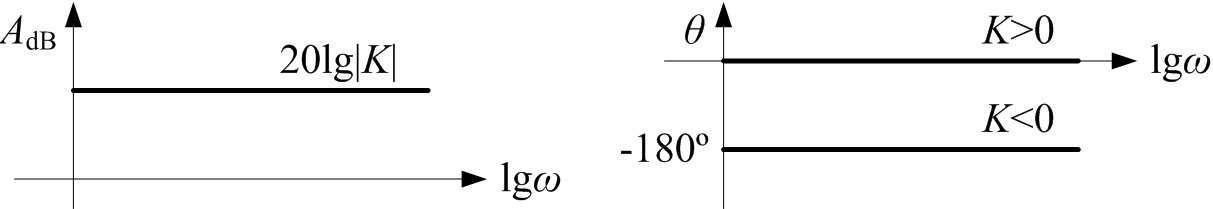
\includegraphics[height=1.8cm]{8.4.2-1.png}
\end{figure}
\[
A_{\mathrm{dB}}=20\lg \left| K \right| \qquad \qquad \theta =\mathrm{arc}\tan \frac{0}{K}=\begin{cases}
	0 &K>0\\
	-\pi &K<0\\
\end{cases}
\]

~

{\bf 因子$i\omega $}

当出现在分子多项式中时,增益为斜率20dB/10倍频的过$\left( 1,0 \right) $的上升直线,相位稳定在$\pi /2$。

\begin{figure}[ht]
\centering
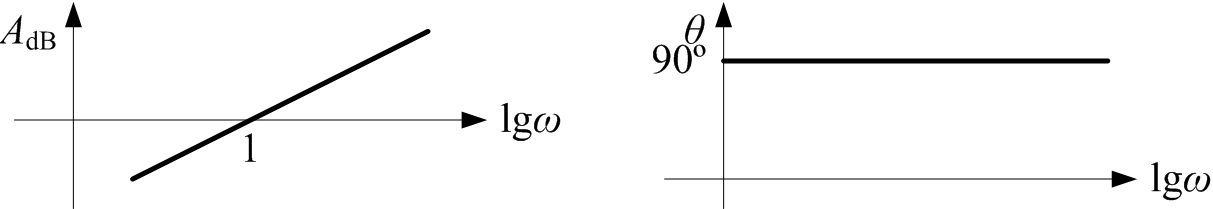
\includegraphics[height=1.8cm]{8.4.2-2.png}
\end{figure}
\[
A_{\mathrm{dB}}=20\lg \left| i\omega \right|=20\lg \omega \qquad \qquad \theta =\mathrm{arc}\tan \frac{\omega}{0}=\frac{\pi}{2}
\]

当出现在分母多项式中时,增益为斜率-20dB/10倍频的过$\left( 1,0 \right) $的下降直线,相位稳定在$-\pi /2$。
\begin{figure}[h]
\centering
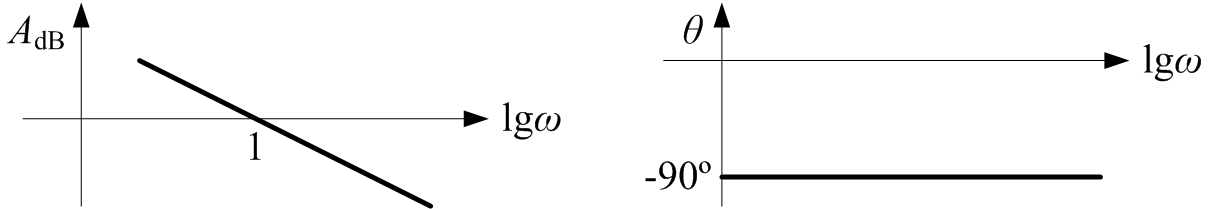
\includegraphics[height=1.8cm]{8.4.2-3.png}
\end{figure}
\[
A_{\mathrm{dB}}=20\lg \left| \frac{1}{i\omega} \right|=-20\lg \omega \qquad \qquad \theta =-\mathrm{arc}\tan \frac{\omega}{0}=-\frac{\pi}{2}
\]

{\bf 因子$i\frac{\omega}{\omega _z}+1$}

当出现在分子多项式中时,增益为0的平行线,过了转角频率 后为斜率为20dB/10倍频的上升直线,相位起初为0,转角频率$\omega _z$处达到$\pi /4$,最后稳定在$\pi /2$。
\begin{figure}[h]
\centering
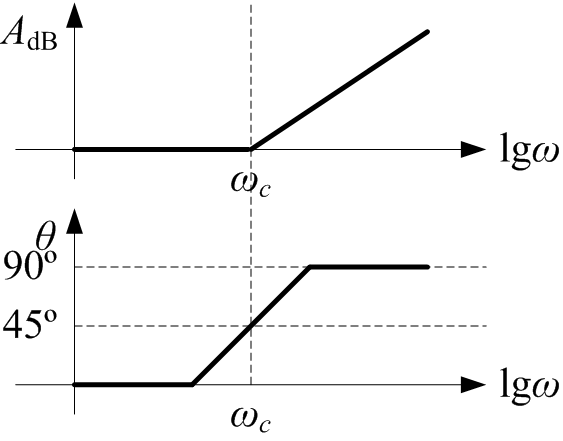
\includegraphics[height=3.5cm]{8.4.2-4.png}
\end{figure}
\begin{align*}
&A_{\mathrm{dB}}=20\lg \left| i\frac{\omega}{\omega _z}+1 \right|=20\lg \sqrt{\left( \frac{\omega}{\omega _z} \right) ^2+1}=\begin{cases}
	0 &\omega <\omega _z\\
	20\lg \frac{\omega}{\omega _z} &\omega >\omega _z\\
\end{cases} \\
&\theta =\mathrm{arc}\tan \frac{\omega}{\omega _z}=\begin{cases}
	0 &\omega <\frac{\omega _z}{10}\\
	\frac{\pi}{4} &\omega =\omega _z\\
	\frac{\pi}{2} &\omega >10\omega _z\\
\end{cases}
\end{align*}

当出现在分子多项式中时,增益为0的平行线,过了转角频率 后为斜率为-20dB/10倍频的下降直线,相位起初为0,转角频率$\omega _z$处达到$-\pi /4$,最后稳定在$-\pi /2$。
\begin{figure}[ht]
\centering
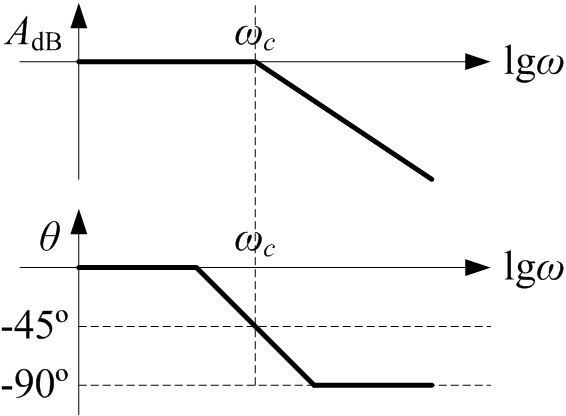
\includegraphics[height=3.5cm]{8.4.2-5.png}
\end{figure}
\begin{align*}
&A_{\mathrm{dB}}=20\lg \frac{1}{\left| i\frac{\omega}{\omega _p}+1 \right|}=-20\lg \sqrt{\left( \frac{\omega}{\omega _p} \right) ^2+1}=\begin{cases}
	0 &\omega <\omega _p\\
	-20\lg \frac{\omega}{\omega _p} &\omega >\omega _p\\
\end{cases} \\
&\theta =-\mathrm{arc}\tan \frac{\omega}{\omega _z}=\begin{cases}
	0 &\omega <\frac{\omega _p}{10}\\
	-\frac{\pi}{4} &\omega =\omega _p\\
	-\frac{\pi}{2} &\omega >10\omega _p\\
\end{cases}
\end{align*}

%============================================================
\subsection{Python应用——scipy.signal.bode函数}

scipy.signal.bode()函数用于生成系统的波特图。
\begin{figure}[h]
\centering
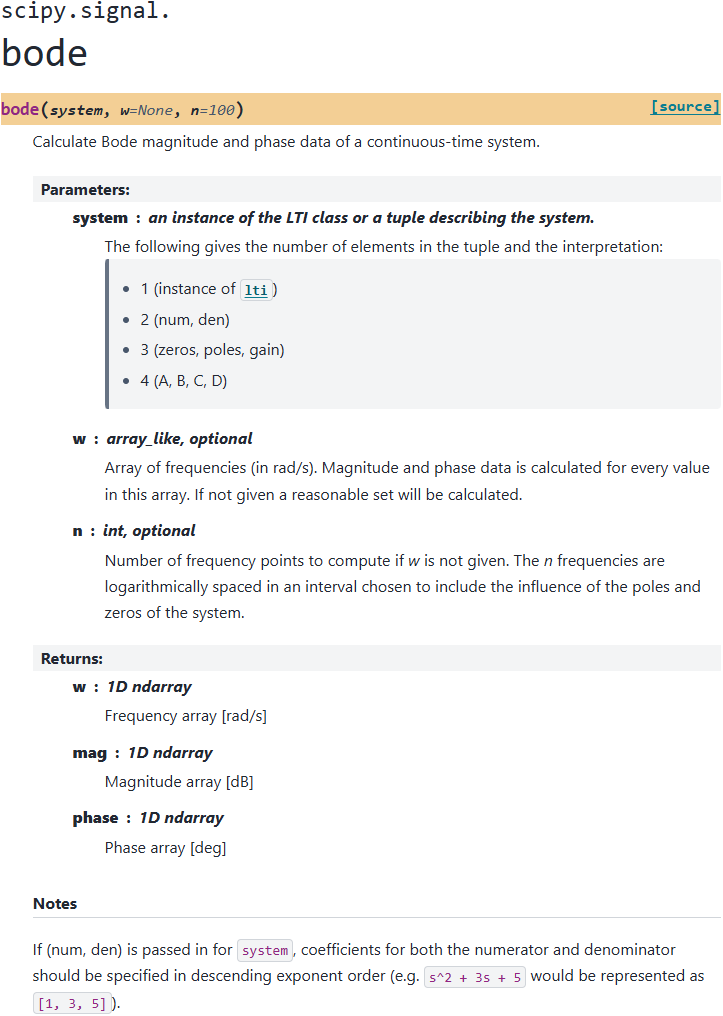
\includegraphics[width=7.5cm]{8.4.3-1.png}
\end{figure}

~

\begin{example}
若系统传递函数$H\left( s \right) =\frac{2}{s+2}$,画波特图。
\end{example}

\begin{python}
H = signal.TransferFunction([2], [1,2])
w = np.arange(0.1, 100, 0.01)
w, mag, phase = H.bode(w=w)

axs[0][0].plot(w, mag);   axs[0][0].set_xscale('log')
axs[1][0].plot(w, phase); axs[1][0].set_xscale('log')
axs[0][1].plot(w, mag)
axs[1][1].plot(w, phase)
\end{python}

\begin{figure}[h]
\centering
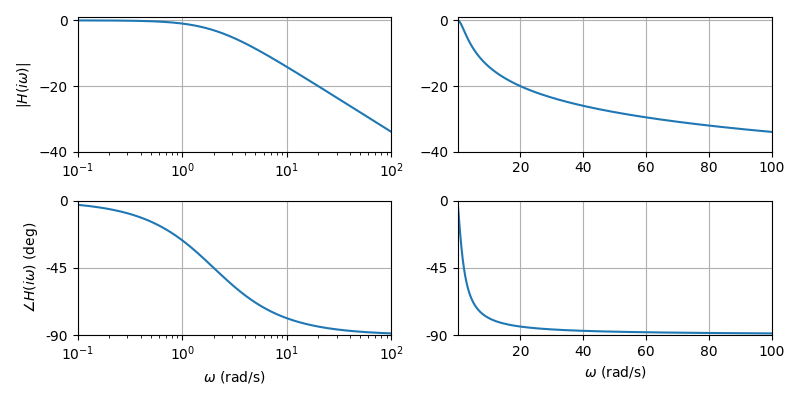
\includegraphics[height=5cm]{8.4.3-2.png}
\end{figure}




